\documentclass[UTF8,a4paper,zihao=5]{ctexart}
\usepackage{geometry}
\usepackage{indentfirst}
\usepackage{setspace}
\usepackage{amsmath,amssymb}
\usepackage{booktabs}
\usepackage{graphicx}
\usepackage{float}
\usepackage{caption}
\usepackage{hyperref}
\usepackage{enumitem}
\usepackage{titlesec}
\usepackage[superscript,sort,compress]{cite}
\makeatletter
\renewcommand{\@cite}[2]{\textsuperscript{[#1\if@tempswa , #2\fi]}}
\makeatother
\hypersetup{
  hidelinks,
  pdfborder={0 0 0}
}

\geometry{a4paper,left=2.4cm,right=2.4cm,top=2.4cm,bottom=2.4cm}
\setstretch{1.5}
\AtBeginDocument{\setlength{\parindent}{2\ccwd}}
\setlist[itemize]{itemsep=2pt, parsep=0pt, topsep=4pt}
\setlist[enumerate]{itemsep=2pt, parsep=0pt, topsep=4pt}
\titlespacing*{\section}{0pt}{0.9\baselineskip}{0.5\baselineskip}
\titlespacing*{\subsection}{0pt}{0.7\baselineskip}{0.35\baselineskip}

\title{面向软件版权存证的双指纹风险分流方法与实现\\（论文大纲）}
\author{作者姓名\thanks{作者单位，邮箱：xxx@xxx.com}}
\date{\today}

\begin{document}
\maketitle
\vspace{-0.6\baselineskip}

\begin{abstract}
【研究背景】软件版权存证场景中，传统单一文件哈希难以识别“改注释/改格式”的近似重复提交。\\
【研究问题】如何在保证实时性和可审计性的前提下，实现低成本风险筛查与人工复核分流。\\
【核心方法】提出双指纹机制（\texttt{normalizedHash} + \texttt{semanticHash}），并基于相似度阈值实现风险分流。\\
【系统实现】结合后端申请状态机（\texttt{PENDING\_REVIEW}、\texttt{ONCHAIN\_SUCCESS} 等）完成链上链下协同。\\
【实验设计】从准确性、人工复核负担和处理时延三个维度进行对比与消融验证。
\end{abstract}

\noindent 关键词：软件版权存证；双指纹；风险分流；人工复核；区块链审计

\vspace{0.4em}
\noindent Abstract: This outline focuses on a dual-fingerprint triage method for software copyright evidence submission.
It combines strict normalized digest matching and semantic digest similarity to support practical risk routing
between auto-pass and manual review under auditable state transitions.

\section{引言}
\subsection{研究背景、必要性与相关性}
随着软件资产化和在线登记流程的普及，版权存证系统需要同时满足“处理效率、风险识别和证据可信”三类目标\cite{r1,r4,r5}。在实际业务中，提交对象往往是压缩包或多文件归档，既存在完全重复提交，也存在通过注释、空白或目录微调进行“表层改写”的近似重复提交\cite{r2,r3}。若仅依赖原始文件哈希，系统虽能高效识别字节级重复，却难以有效覆盖后者；若完全依赖人工复核，则会显著增加审核负担并拉长处理周期。因此，构建一种可在工程场景中低成本运行、又能支撑审计回放的风险分流机制具有现实必要性。

\subsection{研究目标}
面向高并发的软件版权存证场景，系统既需要保持提交处理效率，又要尽可能识别近似改写带来的潜在风险，并为后续复核与争议处理提供可追溯依据。现有做法中，单一文件哈希适合快速判重，但对表层改写样本识别能力有限；完全依赖人工审核虽然灵活，却容易在规模增长时带来明显的人力与时延压力。

基于上述现实约束，本文的目标是在不显著增加系统开销的前提下，构建一种可工程落地的风险筛查机制：通过双指纹协同提升风险样本捕获能力，通过分流规则平衡自动处理与人工复核负担，并在链上链下协同流程中保留可审计、可回放的关键证据与状态信息。

\subsection{主要贡献与方法概览}
本文提出并实现了面向软件版权存证场景的双指纹风险分流方法，其中以 \texttt{normalizedHash} 完成严格判重，以 \texttt{semanticHash} 支撑近似检测，在识别能力与计算开销之间取得平衡；在此基础上，系统结合相似度阈值与主体关系构建风险分流策略，将申请路由至自动上链或人工复核，并通过链下业务状态机与链上摘要锚定协同实现结果追踪与审计回放。研究方法上，本文采用“规则驱动的工程实现 + 实验评估”的技术路径，即先完成方法建模与系统落地，再通过对比与消融实验从识别效果、复核负担和处理时延三个维度进行量化验证。与本主题相关的既有工作仅在本节作背景性提及，详细讨论放在第2节展开。

\section{相关工作}
\subsection{哈希去重与软件制品治理}
围绕软件制品治理，已有研究与工程实践普遍采用基于哈希的内容寻址与去重机制，以保证数据完整性并降低重复存储成本\cite{r1}。这类方法在“字节级一致”判断上具有高效率和高确定性，适合构建上传门禁中的第一道校验。然而，版权存证场景中的风险并不只来源于完全重复样本，许多高风险提交体现为结构或语义近似但字节不一致，单哈希机制在此类样本上的识别能力有限。本文在继承其高效判重优势的基础上，进一步引入面向近似样本的补充判定机制。

\subsection{代码相似性检测方法}
代码相似性检测领域已形成从文本级、词法级到语法/语义级的多层方法体系\cite{r2,r3}，能够在学术评测或离线分析中提供较强的相似识别能力。相关方法在精度上具有优势，但在高并发业务门禁场景中，往往面临计算代价高、结果解释复杂、与在线流程耦合难等问题。与这类工作相比，本文不追求“最深层语义还原”，而是聚焦于可在线部署的风险分流目标：以较低成本快速筛出需要人工介入的高风险样本，并将规则与状态迁移显式化，以便审计和复核。

\subsection{区块链存证与可审计性}
在版权保护与电子证据管理中，区块链存证通常用于提供时间戳、不可篡改记录与跨方可验证能力\cite{r4,r5}。现有方案多强调“确权证明”或“证据保全”，但对“存证前风险筛查”与“审核工作量控制”的关注相对不足。本文在链上锚定思路上进行拓展：不仅保存关键摘要，还将风险分流结果与状态流转过程纳入可追溯链路，使链上能力从“结果证明”进一步延伸到“过程审计”。

综合来看，已有工作分别在强一致判重、深度相似检测与可信存证方面提供了重要基础，但尚缺少一种能够在版权存证业务中同时兼顾在线效率、风险分流和流程可审计性的统一方案。本文正是在这一空白上展开：通过双指纹协同判定连接“高效筛查”与“近似识别”，通过阈值分流连接“自动处理”与“人工复核”，并通过链上链下协同连接“业务执行”与“证据回放”。

\section{双指纹风险分流方法}
\subsection{整体流程}
本文方法与系统实现保持一致，输入为上传文件、软件名称与描述字段，输出为申请状态、风险结论与链上回执信息。流程上，系统首先完成文件接收、主体身份校验与申请编号生成（格式为 \texttt{APP-时间戳-8位随机后缀}），随后在同一事务中执行指纹构建、风险评估与分流决策。若命中人工复核条件，则仅落库申请与证据并返回 \texttt{PENDING\_REVIEW}；若未命中复核条件，则继续执行链上登记并在成功后生成正式版权记录。该流程的设计目标是将“筛查决策”与“确权执行”解耦，以降低错误上链和重复上链风险。

在进入相似度评估前，系统执行两类前置去重约束：其一，按 \texttt{fileHash} 检查正式版权记录是否已存在；其二，按 \texttt{normalizedHash} 检查规范化归档是否已存在证据记录。双约束组合能够同时覆盖“完全重复提交”和“结构一致重打包”两类常见重复风险。

\begin{center}
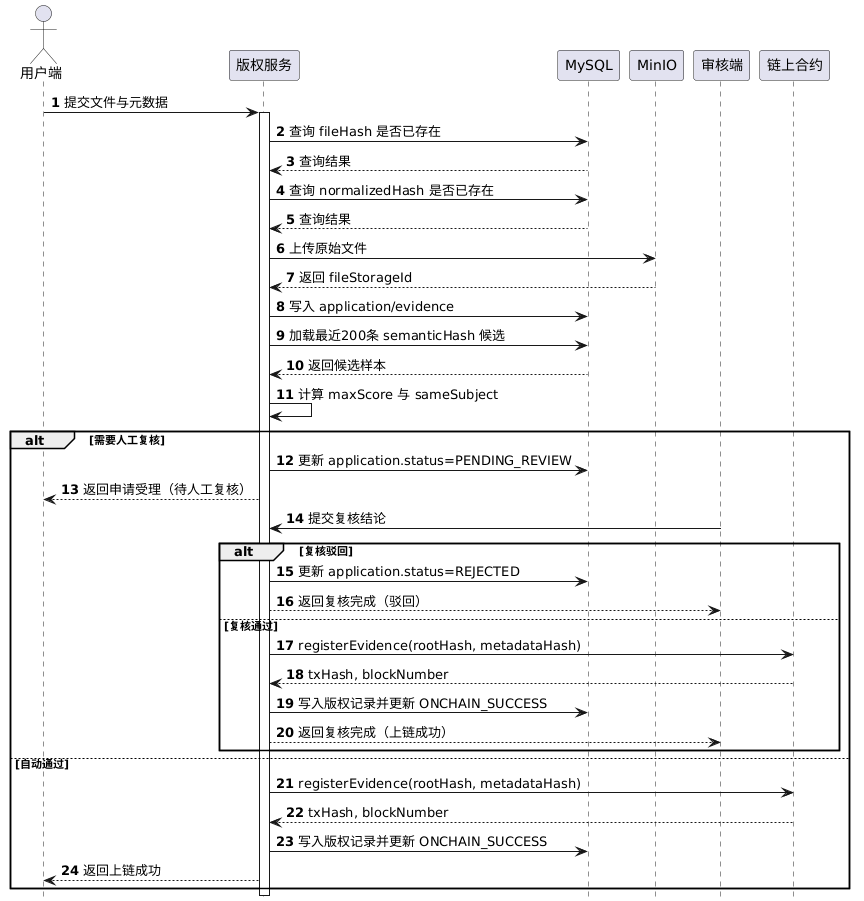
\includegraphics[width=0.95\textwidth]{figures/shixu.png}
\captionof{figure}{业务时序图}
\label{fig:business-sequence}
\end{center}

\subsection{双指纹定义}
系统采用双指纹机制：\texttt{normalizedHash} 用于强一致判定，\texttt{semanticHash} 用于近似检测。具体实现中，\texttt{ArchiveFingerprintUtils} 会先尝试解压归档并提取“路径-内容”映射，按路径排序后构建两类摘要串。对规范化摘要，系统拼接“标准化路径 + 原始内容Base64”后计算 SHA-256；对语义摘要，系统对文本文件执行去注释、压缩空白等归一化，再拼接“标准化路径 + 归一化内容”计算 SHA-256。非文本文件不做文本归一化，而是直接引入其原始字节摘要，避免二进制误解码噪声。

除双指纹外，系统还构建元数据摘要和证据根摘要，用于链上登记与证据绑定。令上传文件字节为 $F$，软件名与描述拼接后的元数据串为 $M$，则有：
\begin{equation}
H_{\mathrm{file}}=\mathrm{SHA256}(F), \quad
H_{\mathrm{meta}}=\mathrm{SHA256}(M), \quad
H_{\mathrm{root}}=\mathrm{SHA256}(H_{\mathrm{file}} \parallel H_{\mathrm{meta}}).
\end{equation}
其中 $H_{\mathrm{root}}$ 作为链上登记的核心证据键，保证文件内容与业务元数据在证据层的绑定关系。

\begin{equation}
H_{\mathrm{norm}} = \mathrm{SHA256}\left(\mathrm{normalize}(archive)\right)
\end{equation}
\begin{equation}
H_{\mathrm{sem}} = \mathrm{SHA256}\left(\mathrm{semantic\_normalize}(archive)\right)
\end{equation}

\subsection{风险分流规则}
相似度评估以最近历史样本为范围进行，系统从 \texttt{copyright\_records} 中读取 \texttt{semanticHash} 非空的最新 200 条记录（\texttt{SIMILARITY\_SCAN\_LIMIT=200}），逐条计算当前样本与候选样本的哈明距离分值，并取最大分值作为本次判定依据。评分实现与代码一致，可写为：
\begin{equation}
S = \mathrm{clip}\left(\mathrm{round}\left(100 \times \left(1-\frac{d_H(h_a,h_b)}{L}\right)\right),0,100\right),
\end{equation}
其中 $d_H$ 为哈明距离，$L$ 为比特长度。

系统采用双阈值分流：高风险阈值 $T_h=95$，中风险阈值 $T_m=85$。同时引入主体关系修正规则，即在高分条件下区分“同主体版本演进”与“跨主体高相似风险”。设 \texttt{sameSubject} 表示主体一致，则分流策略为：
\begin{align*}
&S \geq 95 \land \neg sameSubject \Rightarrow \text{HIGH，进入 } \texttt{PENDING\_REVIEW};\\
&S \geq 95 \land sameSubject \Rightarrow \text{MEDIUM，可直接进入自动上链};\\
&85 \leq S < 95 \Rightarrow \text{MEDIUM，进入 } \texttt{PENDING\_REVIEW};\\
&S < 85 \Rightarrow \text{LOW，进入自动上链流程}.
\end{align*}
此外，系统在提交入口增加角色约束：企业法务账号禁止发起上链申请，以减少职责冲突与流程越权。

\subsection{状态机与审计字段}
方法的执行语义通过“申请状态 + 链上交易状态”双轨状态机表达。申请主状态包括 \texttt{AUTO\_CHECKED}、\texttt{PENDING\_REVIEW}、\texttt{ONCHAIN\_SUCCESS}、\texttt{ONCHAIN\_FAILED} 和 \texttt{REJECTED}；链上交易状态包括 \texttt{PENDING}、\texttt{SUCCESS}、\texttt{FAILED}。系统在触发上链前先写入一条 \texttt{onchain\_tx(PENDING)} 记录，若链上执行失败则回写 \texttt{FAILED} 并将申请置为 \texttt{ONCHAIN\_FAILED}；若执行成功则回写交易哈希与区块高度，并落正式版权记录，业务状态置为 \texttt{ONCHAIN\_SUCCESS}。

对于人工复核流程，系统仅允许 \texttt{PENDING\_REVIEW} 状态申请进入复核动作：复核驳回时申请状态置为 \texttt{REJECTED} 且不触发上链；复核通过时复用自动流程的上链执行函数，保证“自动通过”和“人工通过”在链上语义与落库结构上的一致性。

审计字段方面，系统在记录层保留相似度分值、风险等级、风险原因、复核结论、复核备注、审核状态、审核人、审核时间以及链上交易凭证等信息，形成从“样本评分”到“最终确权”的全过程追踪链。该设计使方法不仅可用于在线分流，也可支撑事后复核、责任定位与证据回放。

\section{系统实现}
\subsection{实现架构与模块划分}
系统采用前后端分离架构，前端基于 Vue 负责申请提交、状态查询与审核交互，后端基于 Spring Boot 提供统一 API 与状态机执行。后端在服务层按职责拆分为三类核心模块：版权业务模块（申请、风险评估、上链、查询）、认证鉴权模块（登录、主体与角色一致性校验）和企业治理模块（企业成员与法务可见范围管理）。该划分使“业务规则”“权限规则”和“组织治理规则”在代码层保持解耦，便于后续按模块独立演化。

\subsection{后端核心服务实现}
后端核心流程由 \texttt{CopyrightServiceImpl} 实现，关键入口包括 \texttt{submitApplication}、\texttt{reviewApplication}、\texttt{queryByApplicationNo} 等。申请提交流程中，系统在单事务内依次完成文件哈希与双指纹生成、重复性校验、对象存储写入、申请与证据落库、风险评分与分流决策；在非复核路径下继续执行上链并写入正式版权记录。为保证业务可追溯性，上链动作通过独立的 \texttt{onchain\_tx} 记录维护 \texttt{PENDING/SUCCESS/FAILED} 执行状态，并与申请状态联动更新。

鉴权与主体模型由 \texttt{AuthServiceImpl} 和 \texttt{AuthDomainRules} 协同实现。系统在登录阶段对账号主体与角色兼容性进行校验，统一签发 JWT，并在请求过滤阶段写入安全上下文。企业侧管理由 \texttt{EnterpriseMemberServiceImpl} 负责，所有成员写操作都被限制在当前企业管理员所属 \texttt{enterpriseId} 范围内，从服务层防止跨企业越权。

\subsection{前端业务编排与交互逻辑}
前端通过 API 分层封装业务请求，并在路由守卫中按“登录态-平台角色-企业角色-法务范围”顺序执行访问控制。申请页在提交后先获得申请编号与初始状态，再对中间态进行定时轮询，直到进入 \texttt{ONCHAIN\_SUCCESS} 或 \texttt{ONCHAIN\_FAILED} 等终态。审核页围绕待审核列表、通过/驳回动作构建审核闭环；管理页与企业成员页分别承载平台级账号治理和企业内部成员治理。该编排方式使前端交互语义与后端状态机保持一致，减少了页面状态与业务状态不一致的问题。

\subsection{链上链下协同与一致性保障}
系统采用“链下存原文、链上存摘要”的协同模式。链下部分由 MySQL 与 MinIO 共同维护完整证据链：\texttt{file\_storage} 保存原文件位置，\texttt{copyright\_application} 与 \texttt{copyright\_evidence} 保存申请和指纹证据，\texttt{copyright\_records} 保存确权结果；链上部分通过 FISCO BCOS 合约 \texttt{registerEvidence} 写入证据根摘要并返回交易回执。为降低重复登记风险，系统在调用上链前先查询链上是否已存在同一证据根；若交易失败则保留失败信息并回写 \texttt{ONCHAIN\_FAILED}，避免“状态成功但链上失败”的伪一致。

\section{实验设计与结果分析}
\subsection{数据集与样本构造}
\begin{itemize}[leftmargin=2em]
  \item 样本规模：\underline{\hspace{2.0cm}} 个；
  \item 近似改写样本比例：\underline{\hspace{2.0cm}}；
  \item 跨主体高相似样本比例：\underline{\hspace{2.0cm}}。
\end{itemize}

\subsection{对比方案}
\begin{itemize}[leftmargin=2em]
  \item Baseline-1：仅 \texttt{fileHash}；
  \item Baseline-2：仅 \texttt{semanticHash}；
  \item Ours：双指纹 + 风险分流 + 状态机闭环。
\end{itemize}

\subsection{评价指标}
\begin{itemize}[leftmargin=2em]
  \item 识别能力：Precision / Recall / F1；
  \item 运营指标：人工复核率、误报率、漏报率；
  \item 性能指标：平均处理时延、吞吐量。
\end{itemize}

\subsection{消融与敏感性实验}
\begin{itemize}[leftmargin=2em]
  \item 去除 \texttt{normalizedHash} 的影响；
  \item 去除“跨主体加权规则”的影响；
  \item 阈值 $T_h,T_m$ 对复核负担和准确率的影响。
\end{itemize}

\subsection{结果呈现模板}
\begin{itemize}[leftmargin=2em]
  \item 表1：主对比结果（Baseline vs Ours）；
  \item 表2：消融实验结果；
  \item 图1：阈值-复核率-准确率权衡曲线。
\end{itemize}

\section{结论与展望（提纲）}
\begin{itemize}[leftmargin=2em]
  \item 总结双指纹分流机制对版权存证效率与可靠性的提升。
  \item 强调“自动分流不替代法律鉴定”，人工复核仍为关键闭环。
  \item 展望：引入更强语义特征、跨项目迁移评估、动态阈值学习。
\end{itemize}

\vspace{0.4em}
\noindent\textbf{致谢（占位）}：感谢\underline{\hspace{5cm}}。

\begin{thebibliography}{99}
\bibitem{r1} 文献占位1：哈希去重与软件供应链治理。
\bibitem{r2} 文献占位2：代码相似性检测综述。
\bibitem{r3} 文献占位3：局部敏感哈希与近重复检测。
\bibitem{r4} 文献占位4：区块链存证与审计机制。
\bibitem{r5} 文献占位5：软件版权与司法鉴定规范。
\end{thebibliography}

\end{document}
